%%%%%%%%%%%%%%%%%%%%%%%%%%%%%%%%%%%%%%%%%%%%%%%%%%%%%%%%%%%%%%%%%
%
%   Circle Packing Research Poster
%   Created with LaTeX using the beamerposter package.
%   This template is designed to highlight key research contributions.
%
%%%%%%%%%%%%%%%%%%%%%%%%%%%%%%%%%%%%%%%%%%%%%%%%%%%%%%%%%%%%%%%%%

\documentclass[final]{beamer}
% Use beamerposter package with portrait orientation, A0 size, and increased scale for larger font
\usepackage[orientation=landscape, size=a0, scale=1.4]{beamerposter}
\usepackage{graphicx} % Required for including images
\usepackage{amsmath}  % For advanced math environments
\usepackage{amssymb}  % For math symbols like \mathbb
\usepackage{booktabs} % For professional quality tables
\usepackage{caption}  % For captions outside floats

% Define custom colors for blocks to make them stand out
\usecolortheme{rose}
\setbeamercolor{block title}{bg=blue!20!white,fg=black}
\setbeamercolor{block body}{bg=blue!10!white,fg=black}
\setbeamercolor{block title alerted}{bg=red!30!white,fg=black}
\setbeamercolor{block body alerted}{bg=red!10!white,fg=black}
% Set a background color for the main title header
\setbeamercolor{title in head/foot}{bg=blue!15!white}


% --- Poster Title, Author, and Institute ---
\title{Circle Packing and the Discrete Schwarz Lemma}
\author{Arham Lodha}
\institute{DIMACS REU Program, Rutgers University}



% --- Document Start ---
\begin{document}

% The entire poster content, including the header, must be inside a single frame environment
% to prevent page breaks. The [t] option aligns content to the top.
\begin{frame}[t]

    % --- Poster Header ---
    % Reverting to the original structure with a new, simpler 3-column layout.
    \nointerlineskip
    \makebox[\linewidth][c]{%
        \begin{beamercolorbox}[wd=\paperwidth, left=2cm, right=2cm]{title in head/foot}
            \vspace*{1cm} % Vertical padding
            \begin{columns}[T, totalwidth=\textwidth]
                % === LEFT LOGO ===
                \begin{column}{0.15\textwidth}
                    \centering
                    
\includegraphics[height=5cm]{nsf-logo.png}
                \end{column}

                % === CENTERED TEXT ===
                \begin{column}{0.7\textwidth}
                    \centering
                    {\huge\textbf{\inserttitle}\par}
                    \vspace{0.5cm}
                    {\large\insertauthor\par}
                    \vspace{0.25cm}
                    {\normalsize\insertinstitute\par}
                \end{column}

                % === RIGHT LOGO ===
                \begin{column}{0.15\textwidth}
                    \centering
                    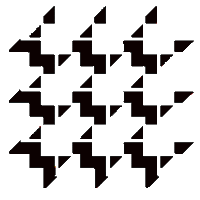
\includegraphics[height=5cm]{dimacs-logo.png}
                \end{column}
            \end{columns}
            \vspace*{1cm} % Vertical padding
        \end{beamercolorbox}%
    }

    % --- Main Content Columns ---
    \begin{columns}[T] % The main content is organized in columns

        % === COLUMN 1: INTRODUCTION & PREVIOUS WORK ===
        \begin{column}{0.32\linewidth}

            % --- Introduction Block ---
            \begin{block}{Introduction}
                The study of circle packings provides a discrete analog to classical complex analysis. By assigning radii to vertices of a triangulated surface, we can define geometric structures like edge lengths and curvature. This framework allows us to explore discrete versions of fundamental theorems like the Schwarz Lemma.
            \end{block}

            % --- Definitions Block ---
            \begin{block}{Core Concepts}
                \textbf{Triangulated Surface $(S, \mathcal{T})$:} A surface $S$ decomposed into a set of triangles $\mathcal{T}$.
                \vspace{1em}

                \textbf{Circle Packing Metric:} A radius function $r: V \to (0, \infty)$ where the induced edge lengths satisfy the triangle inequality for every face in $\mathcal{T}$. For tangent circles, edge lengths are $l_{ij} = r_i + r_j$.
                \vspace{1em}

                \textbf{Discrete Curvature:} For a vertex $v_i$, the curvature is the angle defect:
                $$ K_r(v_i) := 2\pi - \sum_{ijk \in F} \theta_i^{jk} $$
                where $\theta_i^{jk}$ is the angle at vertex $v_i$ in the triangle $(i,j,k)$.

                \begin{center}
                    \includegraphics[width=0.8\linewidth]{discretecurvature.jpg}
                    \captionof{figure}{Discrete curvature as angle defect.}
                \end{center}
            \end{block}

            % --- Previous Work Block ---
            \begin{block}{Previous Work: Rigidity and the Schwarz Lemma}
                \textbf{Thurston's Rigidity Theorem (1985):}
                If two circle packing metrics $R$ and $r$ on a closed triangulated surface have the same discrete curvature ($K_R = K_r$), then they are related by a constant scaling factor ($R = \lambda r$).
                \vspace{1em}

                \textbf{Discrete Schwarz-Pick Lemma (Beardon & Stephenson, 1991):}
                Let $(S, \mathcal{T})$ be a closed triangulated surface with vertices partitioned $V = V_1 \sqcup V_2$. If $R$ and $r$ are circle packing metrics such that:
                \begin{itemize}
                    \item $K_R(v) \ge K_r(v)$ for all $v \in V_1$
                    \item $R(v) \ge r(v)$ for all $v \in V_2$
                \end{itemize}
                Then $R(v) \ge r(v)$ for all $v \in V$.
            \end{block}

        \end{column}

        % === COLUMN 2: MAIN THEOREM & METHODOLOGY ===
        \begin{column}{0.32\linewidth}

            % --- Generalization Block ---
            \begin{block}{Generalization: Intersection Angles}
                We generalize the classical circle packing model by allowing adjacent circles to intersect at a prescribed angle, rather than just being tangent.
                \vspace{1em}

                \textbf{Intersection Angles $\Phi$:} A function $\Phi: E \to [0, \pi)$ that assigns an intersection angle to each edge.
                \vspace{1em}

                The edge length $l_{ij}$ is now given by the law of cosines:
                $$ l_{ij}^2 = r_i^2 + r_j^2 + 2r_i r_j \cos(\Phi_{ij}) $$
            \end{block}

            % --- MAIN THEOREM BLOCK ---
            % Using an "alertblock" to draw special attention to this result.
            \begin{alertblock}{Main Theorem 1: Discrete Schwarz Lemma for Intersection Angles}
                Let $(S, \mathcal{T}, \Phi)$ be a closed triangulated surface with intersection angles. Let the vertices be partitioned $V = V_1 \sqcup V_2$.
                \vspace{1em}

                If for every triangle $\triangle v_i v_j v_k$ in the triangulation, the following condition holds for any permutation $\{a, b, c\}$ of $\{i, j, k\}$:
                $$ \cos(\Phi_a) + \cos(\Phi_b)\cos(\Phi_c) \ge 0 $$
                \vspace{1em}

                And if $R$ and $r$ are circle packing metrics such that:
                \begin{itemize}
                    \item $K_R(v) \ge K_r(v)$ for all $v \in V_1$
                    \item $R(v) \ge r(v)$ for all $v \in V_2$
                \end{itemize}
                Then $R(v) \ge r(v)$ for all $v \in V$.
            \end{alertblock}

            \begin{block}{Proof Sketch}
                The proof follows the structure of the original discrete Schwarz lemma but requires re-evaluating the properties of the discrete curvature map. The main challenge is to show that the Jacobian of the curvature map remains an M-matrix under the new condition on intersection angles, which ensures the comparison principle holds.
            \end{block}

        \end{column}

        % === COLUMN 3: COUNTEREXAMPLE & FUTURE WORK ===
        \begin{column}{0.32\linewidth}

            % --- Inversive Distance Block ---
            \begin{block}{Further Generalization: Inversive Distances}
                A further generalization uses inversive distance $I_{ij} \in [1, \infty)$ to define the relationship between circles. The edge length is given by:
                $$ l_{ij}^2 = r_i^2 + r_j^2 + 2r_i r_j I_{ij} $$
                When $I_{ij} = 1$, the circles are tangent. When $I_{ij} > 1$, the circles are separated.
                \vspace{1em}

                \textbf{Conjecture:} The Discrete Schwarz Lemma holds for any inversive distances.
        \end{block}

            % --- COUNTEREXAMPLE BLOCK ---
            % Using an "alertblock" to highlight this key finding.
            \begin{alertblock}{Counterexample for Inversive Distances}
                The conjecture is false. We constructed a counterexample on a simple 4-vertex triangulation. Let $V_1=\{v\}$ and $V_2=\{a,b,c\}$. We define two circle packing metrics, $r$ and $R$.
                \vspace{1em}

                \begin{center}
                    \includegraphics[width=0.9\linewidth]{counterexample.jpeg}
                    \captionof{figure}{The triangulation for the counterexample.}
                \end{center}

                We observe that $R(a) > r(a)$, $R(b) > r(b)$, and $R(c) > r(c)$, and also $K_R(v) > K_r(v)$. However, the conclusion of the Schwarz Lemma fails, as:
                $$ R(v) = 1.47981 < 1.48297 = r(v) $$
                This demonstrates that the Discrete Schwarz Lemma does not hold for arbitrary inversive distances.

                \begin{columns}[T]
                    \begin{column}{0.5\linewidth}
                        \textbf{Metric r:}
                        \tiny
                        \begin{tabular}{lrr}
                        \toprule
                        Vtx & Radius & Curvature \\
                        \midrule
                        a & 1.0 & 2.4930 \\
                        b & 1.0 & 4.5427 \\
                        c & 1.0 & 3.9797 \\
                        v & \textbf{1.4829} & 4.6925 \\
                        \bottomrule
                        \end{tabular}
                    \end{column}
                    \begin{column}{0.5\linewidth}
                        \textbf{Metric R:}
                        \tiny
                        \begin{tabular}{lrr}
                        \toprule
                        Vtx & Radius & Curvature \\
                        \midrule
                        a & 1.0919 & 1.2490 \\
                        b & 2.4579 & 5.2003 \\
                        c & 2.2206 & 4.4997 \\
                        v & \textbf{1.4798} & 4.7589 \\
                        \bottomrule
                        \end{tabular}
                    \end{column}
                \end{columns}
            \end{alertblock}

            % --- Conclusion Block ---
            \begin{block}{Conclusion and Future Work}
                We have successfully extended the Discrete Schwarz Lemma to circle packings with specific intersection angles. However, we have also shown that this lemma does not extend to the more general setting of inversive distances.

                Future work includes:
                \begin{itemize}
                    \item Finding the precise conditions on inversive distances for the lemma to hold.
                    \item Exploring connections to discrete Ricci flow and other geometric analysis on graphs.
                \end{itemize}
            \end{block}

            % --- Acknowledgements and References ---
            \begin{block}{Acknowledgements}
                Thank you to Professor Feng Luo, Professor Hongbin Sun, Dr. Zhenghao Rao, and Mr. Kuijun Liu. This work was supported by the DIMACS REU Program at Rutgers University and NSF Grant \#2220271.
            \end{block}

            \begin{block}{References}
                \footnotesize{
                \begin{enumerate}
                    \item Beardon, A. F., \& Stephenson, K. (1991). The Schwarz-Pick lemma for circle packings. \textit{Illinois Journal of Mathematics}.
                    \item Thurston, W. P. (2022). \textit{The geometry and topology of three-manifolds}. American Mathematical Society.
                    \item Van Eeuwen, J. (1994). The Discrete Schwarz-Pick Lemma for Overlapping Circles. \textit{Proceedings of the American Mathematical Society}.
                \end{enumerate}
                }
            \end{block}

        \end{column}
    \end{columns}
\end{frame}

\end{document}
